\begin{frame}
\frametitle{\charm}
\framesubtitle{}
    \begin{itemize}
        \item description
    \end{itemize}
\end{frame}


\begin{frame}
\frametitle{\charm: Some Capabilities}
\framesubtitle{}
    \begin{itemize}
        \item -
    \end{itemize}
\end{frame}


\begin{frame}
\frametitle{\charm: Portability}
\only<1>{
\framesubtitle{Environments}
    \begin{itemize}
        \item Embedded ARM: cell phones, CARMA dev boards
        \item Commodity x86: servers, desktops, laptops, tablets
        \item Clusters: commodity, with a network
        \item Supercomputers: IBM Blue Gene and POWER, Cray
    \end{itemize}
}
\only<2>{
  \framesubtitle{Operating Systems}
  \begin{itemize}
  \item Linux
  \item Mac OS X
  \item Windows
  \item Proprietary Cray \& IBM
  \end{itemize}
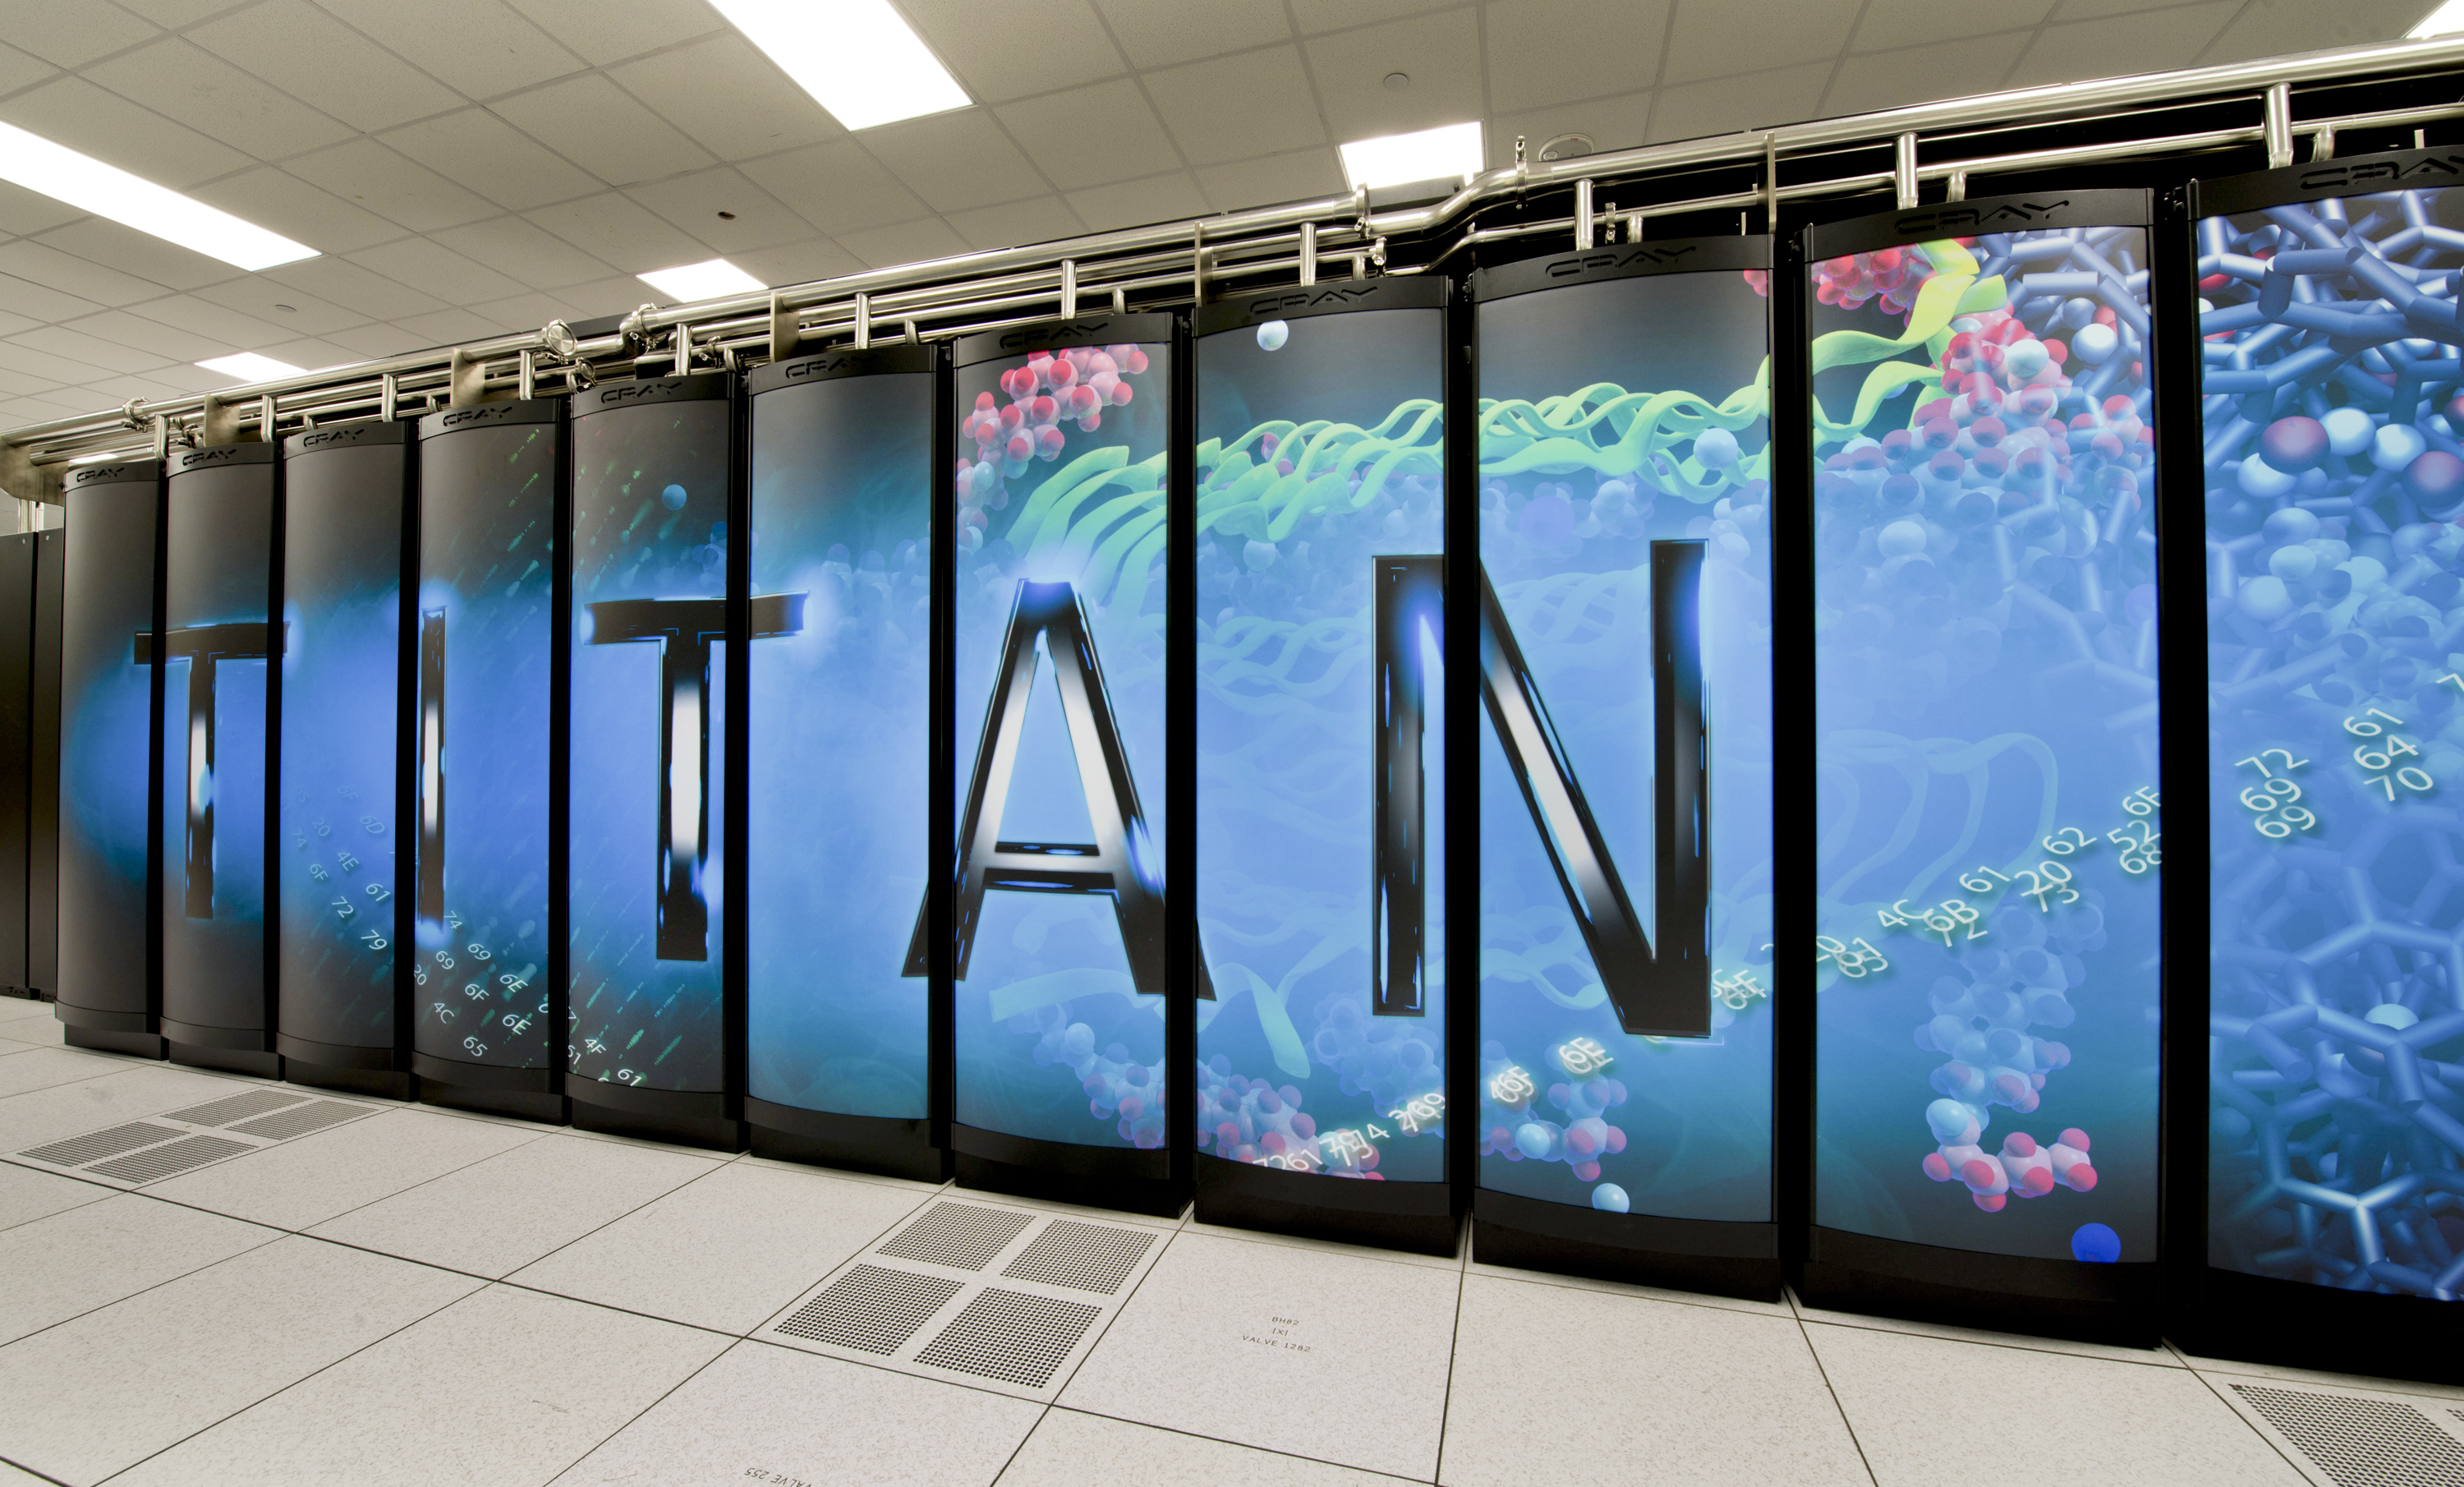
\includegraphics[scale=0.07]{../figures/titan.jpg}
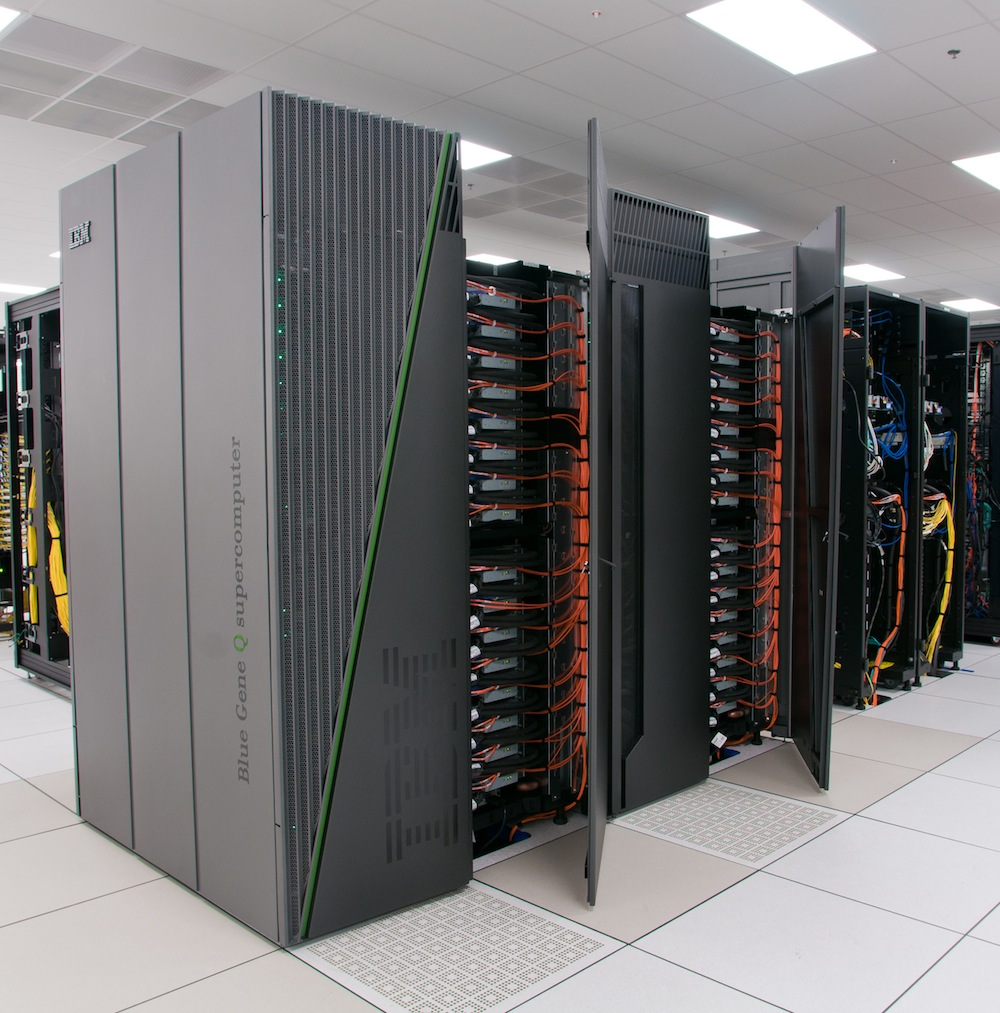
\includegraphics[scale=0.5]{../figures/mira.jpg}
}
\only<3>{
  \framesubtitle{Network Interfaces}
  \begin{itemize}
    \item TCP, UDP
    \item Shared memory
    \item MPI
    \item Infiniband Verbs
    \item Blue Gene P, Q native PAMI
    \item Cray Gemini and Aries native uGNI
  \end{itemize}
}
\only<4>{
\framesubtitle{Compilers}
\begin{itemize}
\item GCC
\item Clang
\item VC++
\item IBM XL
\item Intel
\item PGI
\item Cray
\item Fujitsu
\end{itemize}
}
\end{frame}


